\entry{2026-10-23}{Improvement campaign: final compilation}

All lanes finished; final report \path{reports/2026-10-21-improvement-campaign/final/report.md} (every number traced in \texttt{PROVENANCE.json}; Codex final audit clean). Total 98.46 GPU-h; E4 not run.
\begin{itemize}
\item \textbf{Problem 1, spectral solver faster: partly fixed, box only, under conditions.} Against a dense-matrix spectral FOM, reduced models reach $S\ge2$ only for a narrow family at low steepness, where POD-Galerkin (2.14), POD + ECSW (2.01) and our bank with ETDRK4 (2.07) are equal; the deployed LSPG bank stays at 0.02--0.40. On an L-shape and a box with a hole the bank is 5--70$\times$ slower than POD; a variable coefficient does not slow the FOM enough.
\item \textbf{Problem 2, POD + ECSW dominates: not fixed.} Faster steps raise the worst error slightly; cheaper nonlinear terms fail; the multi-mesh cost claim is withdrawn.
\item \textbf{Problem 3, steep fronts: not fixed.} Retrained banks, finer steps and adaptive quadrature all stop; step certification on steep states is the limit.
\end{itemize}
\begin{center}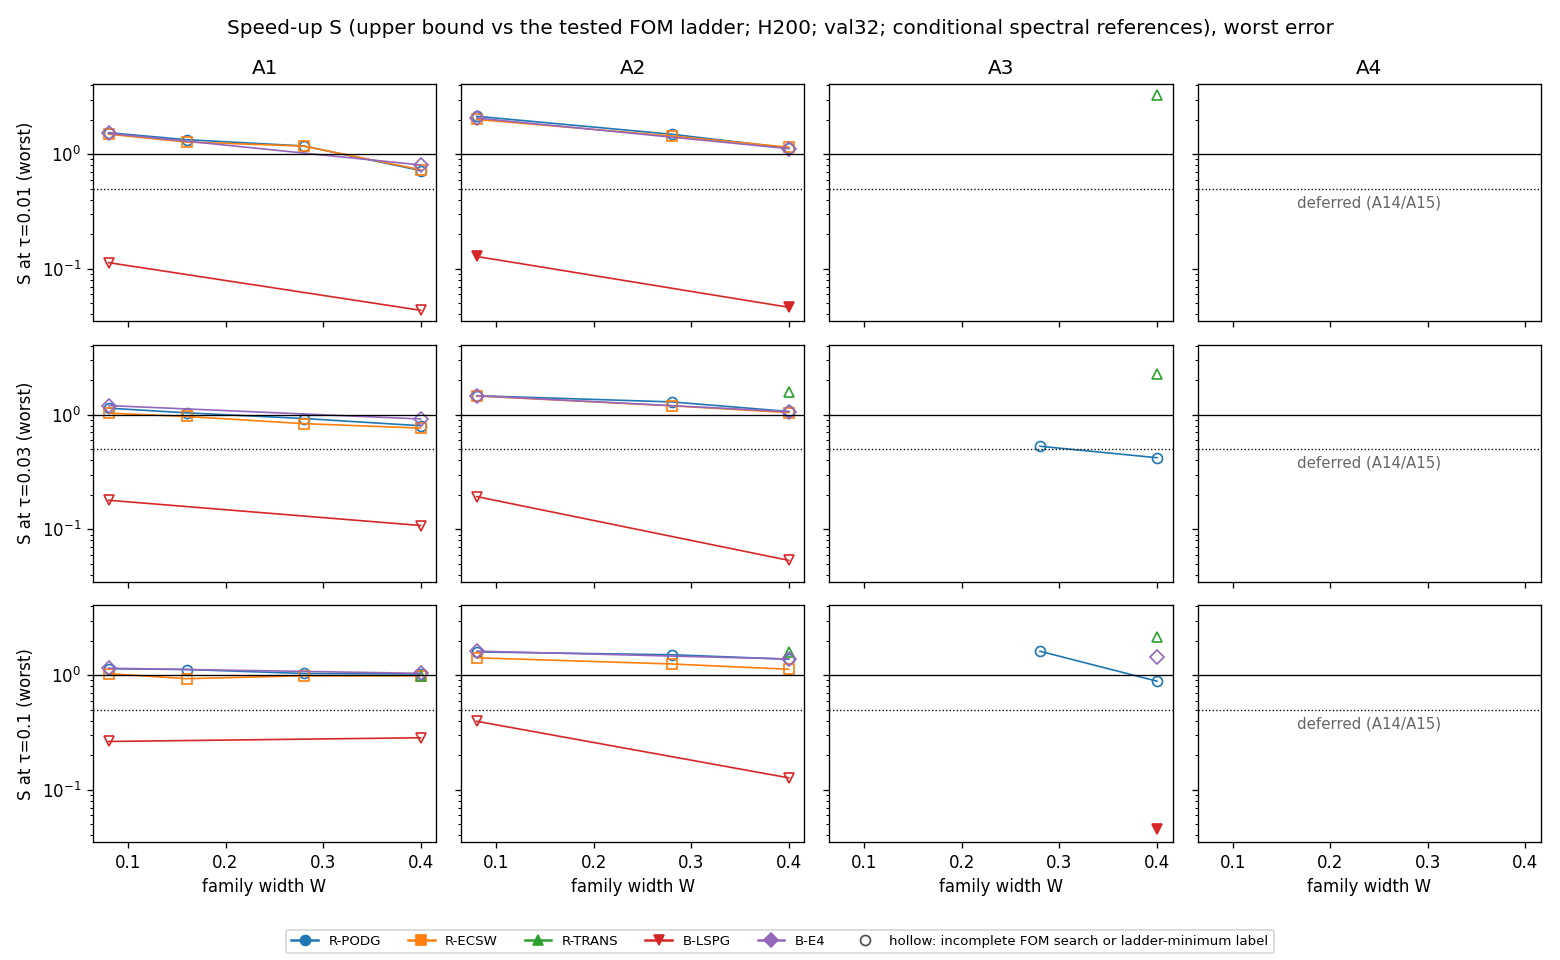
\includegraphics[width=0.48\linewidth]{figs/imp_e1_S_vs_W_worst.png}\hfill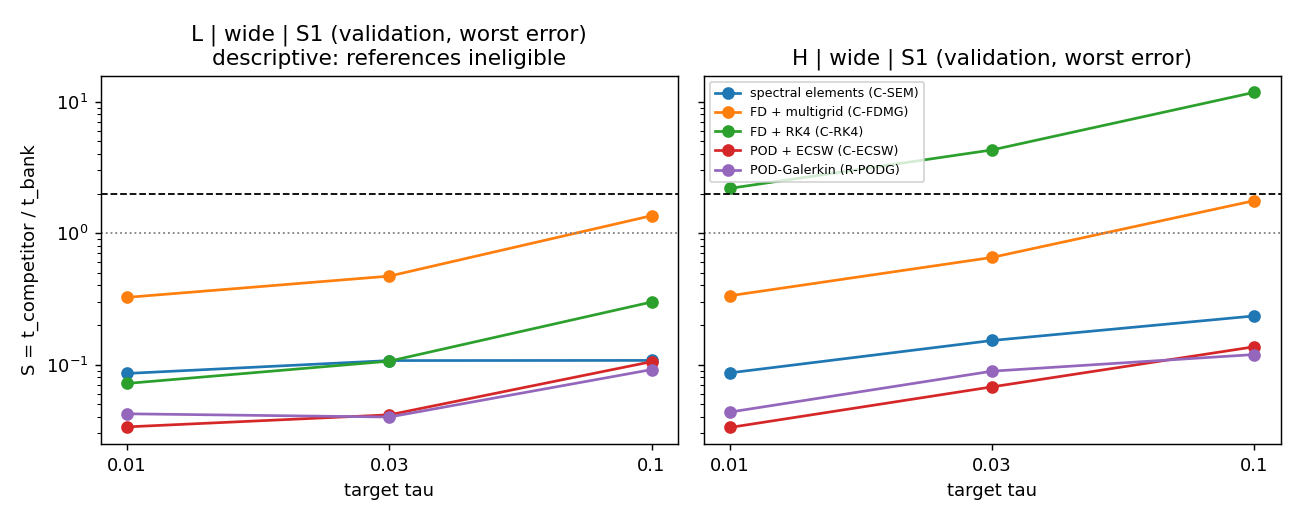
\includegraphics[width=0.48\linewidth]{figs/imp_e2_S_per_family.png}\end{center}
Seven lane branches await the user's merge decision.
